% !TeX spellcheck = ca
\documentclass{article}
\usepackage[utf8]{inputenc}

\usepackage{latexsym}
\usepackage{float}
\usepackage[utf8]{inputenc}
\usepackage[catalan]{babel}
%\usepackage[english]{babel}
\usepackage{microtype}
\usepackage[hyphens]{url}
\usepackage{hyperref}
\usepackage{graphicx}
\usepackage{makeidx}
\usepackage{datetime}
\usepackage{multicol}
\usepackage{setspace}
\usepackage{enumerate}
\usepackage{booktabs}
\usepackage{braket}
\usepackage{listings}
\usepackage{color}
\usepackage{amsmath}
\usepackage{amssymb}
\usepackage[table,xcdraw]{xcolor}
\usepackage{graphicx}
\usepackage{listings}
\usepackage{hyperref}
\usepackage{vmargin}
\usepackage{wrapfig}
\usepackage{subfiles}
\usepackage{float}
\usepackage{amsmath}
\usepackage{amssymb}
\usepackage{tikz-cd}
\usepackage{multirow}
\usepackage{pgffor}
\usepackage{enumitem}
\usepackage{iflang}
\usepackage{varioref}
\usepackage{hyperref}
\usepackage{cleveref}
\usepackage{tikz}
\usepackage{enumitem}


%%%%%%%%%%%%%%%%%%%%%%%%%%%%%%%%%%%%%%%
%%%%%%%%%%%% UTIL COMMANDS %%%%%%%%%%%%  

\setcounter{secnumdepth}{4}
\newcommand{\nc}{\newcommand}
\nc{\supindex}{\textsuperscript}
\renewcommand{\baselinestretch}{1.5}
\nc{\myparagraph}[1]{\paragraph{#1}\mbox{}\\}

%%%%%%%%%%%%%%%%%%%%%%%%%%%%%%%%%%%%%%%
%%%%%%%%%%%%% CONFIG FILE %%%%%%%%%%%%%

\nc{\mytitle}{Implementació d'un sistema criptogràfic per l'enviament del consum en sistemes de comptadors intel·ligents}
\nc{\mysubtitle}{Bayesian Inference}
\nc{\authors}{Oriol Alàs Cercós}
\nc{\datetime}{15\supindex{th} of May, 2020}
\nc{\assignatura}{Treball Final de Grau}
\nc{\professorat}{Francesc Sebé Feixas}

% Per separar professors, utilitzar ','
% 	Ex: Maria, Joan, Pere

%%%%%%%%%%%%%%%%%%%%%%%%%%%%%%%%%%%%%%%
%%%%%%%%%%%%%  LANGUAGE   %%%%%%%%%%%%%

\newcommand{\tr}{\IfLanguageName{english}}

%%%%%%%%%%%%%%%%%%%%%%%%%%%%%%%%%%%%%%%
%%%%%%%%%%%%%%%%% MATH %%%%%%%%%%%%%%%%

\nc{\prob}[1]{P({#1})}
\nc{\probl}[2]{P({#1}|{#2})}

%%%%%%%%%%%%%%%%%%%%%%%%%%%%%%%%%%%%%%%
%%%%%%%%%%%%% TREE CREATOR %%%%%%%%%%%%

\setpapersize{A4}

\author{Oriol Alàs Cercós}
\date{29 d'Abril del 2019}

\def\contentsname{Índex}
\begin{document}
	

\begin{titlepage}
\begin{figure}[htb]
\begin{center}
	
\includegraphics[width=5cm]{imgs/UDL.png}
   	\vspace*{\stretch{1.0}}
   	\\
   	\medskip
   	\begin{center}
   		\medskip\bigskip\bigskip\bigskip
   		
      	\huge\textbf{\mytitle}
      	\\\medskip 	\Large  
      	
      	
      	\bigskip\bigskip\bigskip
      	\bigskip
      	\normalsize{\tr{Made by}{Realitzat per:}}
      	\\
      	\large\textit{\authors}
      	\\
      	\setlength{\parskip}{1em}
      	\normalsize{\tr{Delivery}{Data de lliurament:}}
      	\\
      	\large{\datetime}
   	\end{center}
   	\vspace*{\stretch{2.0}}
\end{center}
\end{figure}
\begin{flushright}
Universitat de Lleida
\\
Escola Politècnica Superior
\\
Grau en Enginyeria Informàtica
\\
\assignatura
\\
\medskip
\textbf{\tr{Professorate:}{Tutor:}}
\\
\foreach \n in \professorat{\n\\}
\end{flushright}
\thispagestyle{empty} 
\end{titlepage}
\tableofcontents
\thispagestyle{empty} 
%\newpage
\listoffigures
\listoftables
\thispagestyle{empty}
\newpage
\part{Introducció}
Els comptadors intel·ligents són dispositius domèstics que recullen i envien 
el consum de l'electricitat a un proveïdor d’energia en intervals de temps reduïts. El consumidor pot saber el seu consum elèctric en tot moment i la seva despesa de manera més precisa amb possibles preus i tarifes personalitzades depenent del consum horari, al permetre la telelectura.
\begin{figure}[H]
	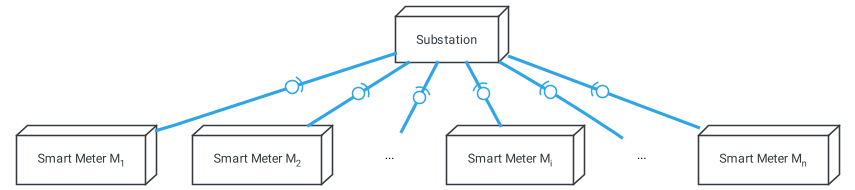
\includegraphics[width=15cm]{umls/network.png}
	\caption{Diagrama de xarxa simple d'un sistema de comptadors.}
\end{figure}
A causa d'aquest constant enviament d'informació,
es poden fer millors prediccions i tendències de consum de manera que la producció pugui estar més a prop de l'energia que es necessita, és a dir, la producció d'energia es pot ajustar més al real consum d'aquesta. A més a més, el distribuïdor d'energia no té la necessitat de revisar manualment el consum i la lectura del comptador elèctric en cada llar.
\\
\\
Tot i que és beneficiosa a gran escala, la quantitat d'informació que proporciona una sola llar es pot utilitzar per fer prediccions de la vida quotidiana \cite{smart-grid-overview}, com per exemple: quan arriben a casa, miren la televisió o se'n van al llit. Per tant, és important mantenir les dades de lectura privades i protegides de qualsevol atac. Arran d'això, s'han realitzat diverses propostes, una d'elles ha estat ideada pel grup de recerca Criptografia i Grafs de la Universitat de Lleida \cite{recsi}.
\\\\
L'objectiu principal d'aquesta memòria ha estat recollir el desenvolupament de la simulació d'aquesta proposta per tal de resoldre el problema anteriorment explicat. No obstant això, es necessita un assoliment dels conceptes que envolten el tema per poder entendre l'actual solució i la seva implementació. Així doncs, els objectius del treball seran:
\begin{itemize}
	\item Estudiar la solució proposada.
	\item Posar en context l'encriptació homomòrfica.
	\item Posar en context l'encriptació ElGamal.
	\item Implementar un client que simuli un comptador intel·ligent.
	\item Implementar un servidor que simuli una subestació d'un barri de comptadors.
	\item Realitzar un estudi dels costs.
\end{itemize}
Abans de submergir-se en detalls de la solució proposada, la \Cref{part:criptografia} s'endinsa en el món de la criptografia i en aquesta s'explica l'encriptació asimètrica i homomòrfica. A més a més, es detalla el sistema en què es basa la nostra proposta, ElGamal. En la \Cref{part:propostes},  s'introdueix una visió general i es plantegen les diferents propostes per tal de solucionar la privacitat dels usuaris. A més a més, s'explica de manera formal el protocol i s'establiran els requeriments. Un cop havent detallat la proposta, es passa a l'explicació de la implementació i el disseny del programa en la \Cref{part:disseny}. Finalment, en la \Cref{part:analisis}  s'analitzarà els costs del programa en funció del nombre de comptadors.
\newpage\part{Criptografia i teoria de la computació}\label{part:criptografia}
\section{Encriptació simètrica i asimètrica}
Un criptosistema està format per dos tipus d'algorismes, un que transforma el
missatge intel·ligible a un altre inintel·ligible i l'altre, de manera inversa. D'aquesta manera, és possible crear una comunicació segura davant de possibles interceptors de la informació maliciosos.
\\
Un criptosistema està constituït per tres conjunts finits i dos famílies de funcions:
\begin{itemize}
	\item El conjunt $M = \{m_1, m_2, ..., m_3\}$ els elements els qual volem xifrar.
	\item El conjunt $C = \{c_1, c_2, ..., c_3\}$ on hi haurà tots aquells elements que poden ser un missatge xifrat.
	\item El conjunt de claus $K$ sobre les quals xifrarem i desxifrarem els missatges.
	\item Funcions d'encriptació $\{E_k \ | \ E_k : M \rightarrow C \}_{k \in K} $
	\item Funcions de desencriptació $\{D_k \ | \ D_k : C \rightarrow M \}_{k \in K}$
\end{itemize}
Aquestes funcions satisfan:
\[ \begin{array}{l}
	\forall \, k_1 \in K, \ \exists \, k_2 \in K\\
	\forall \, m \in M
\end{array} \Bigg\}, \ D_{k_2}(E_{k_1}(m)) = m \Longleftrightarrow D_{k_2} \circ E_{k_1} =  Id\]
Segons la funció d'encriptació i desencriptació, els criptosistemes es poden classificar en dos tipus:
\begin{itemize}
	\item En un criptosistema simètric o convencional, la clau és la mateixa per encriptar com per desencriptar, és a dir, $k_1 = k_2$. Com que l'emisor i el receptor han de compartir la clau, el canal on s'ha de transmetre ha de ser segur perquè no hi hagi interceptors. La seguretat d'aquests sistemes es basen en el gran cost computacional que es requereix per realitzar l'atac de força bruta. Aquest tipus de sistemes es basen en a fer transformacions al missatge a nivell de bit. A diferència de l'encriptació asimètrica, no es poden realitzar signatures digitals, ja que no hi ha distinció de claus entre usuaris.
	\item L'encriptació asimètrica ens proporciona, que tothom o un gran conjunt d'usuaris puguin encriptar el seu missatge, però només un cert conjunt més petit, fins i tot podent ser només un individu, pugui desencriptar el xifrat. Per tal de realitzar això, per encriptar i desencriptar s'utilitzaran dos tipus diferents de claus:
	\begin{itemize}
		\item La \textit{clau pública} s'usarà per xifrar el missatge i la podrà utilitzar qui vulgui.
		\item La \textit{clau privada} s'usara per desxifrar el missatge i només la podrà utilitzar un cert grup d'entitats.
	\end{itemize}
	Aquest tipus de criptosistemes es basen en encriptar mitjançant una funció $c = f(m)$ que sigui fàcil d'evaluar però sigui computacionalment difícil realitzar $f^{-1}(c)$ sense saber una informació addicional que ens permeti trobar el missatge. Aquests tipus de funcions es diuen \textit{trap-door function}.
	Els criptosistemes de clau pública, a diferència dels simètrics, no treballen en nivell de bit, sinó que representen el missatge com un número i realitzen operacions matemàtiques amb ell. 
\end{itemize}

\section{Problema del logaritme discret}
La criptografia que s'utilitzarà en part d'aquest treball es basarà en el problema del logaritme discret.
El problema del logaritme discret és un problema crític en la teoria de nombres i és similar en molts aspectes al problema de la factorització sencera.
\\
\\
Sigui $G$ un grup cíclic finit amb l'operació de multiplicació i l'element d'identitat 1 i $g$ un generador de $G$, llavors cada element $a \in G$ es pot escriure de la forma:
\[a = g^k, \quad k \in \mathbb{Z^+} \] 
Sabent el valor de $a$ i $g$ és computacionalment costós\footnote{És computacionalment costós només en determinats grups, com per exemple: grups cíclics com $Z_p$ o subgrups cíclics de corbes el·líptiques sobre cossos finits. %TODO: explicar quan
} trobar $k$, ja que s'ha de realitzar una búsqueda de totes les possibles solucions fins trobar:
\[k = log_g(a)\]
\subsection{Classificació}

%Tot i que el problema de la descomposició en factors primers i el del logaritme discret són problemes diferents, en cap dels dos es coneix un algorisme eficient si no és realitzat per un ordinador quàntic. Els dos problemes estan catalogats actualment com problemes \textit{NP}  però no estan considerats \textit{NP-Complets} perquè no s'ha trobat una forma de reduir aquests problemes a un problema NP-Complet en temps polinomial.
Encara no s'ha trobat cap algorisme eficient que resolgui el problema del logaritme discret en temps polinomial, per això, actualment pertany al conjunt de problemes \textit{NP}. No obstant això, no està considerat \textit{NP-Complet} ja que no s'ha trobat una forma de reduir aquest problema a un que ja sigui \textit{NP-Complet} en temps polinomial.
\subsection{Pollard's Lambda}
J. M. Pollard \cite{pollard} va descriure dos algoritmes per resoldre el logaritme discret: el mètode \textit{Rho} i el mètode \textit{Lambda} o també anomenat \textit{Kangaroo} \cite{kangaroo}. El mètode \textit{Lambda } relaxa una mica el problema, ja que, donat el grup cíclic $G$, es pretén resoldre el logaritme donat un interval entre uns llindars:
\[g^k = a, \quad L \le k \le U\]
Per tal de resoldre-ho, es creen dos seqüències que, al trobar-se en un punt vol dir que s'ha trobat la potència que s'està buscant. El perquè del nom d'aquest mètode esdevé d'una metàfora, que rau en dos cangurs (les seqüències), un mans i l'altre salvatge. Aquests es situen en un punt que sabem i en un que no, que serà el que voldrem saber, respectivament. Quan vagin saltant i es trobin, sabent el comportament del salvatge podrem veure a quin punt estava situat al principi.
\begin{enumerate}
	\item S'escolleix una funció $f$ pseudoaleatòria que mapejarà els elements del grup a un conjunt petit d'enters positius $S$ denominats els salts:
	\[f : G \rightarrow S, \qquad S = \{s_1, \dots, s_n\}\]
	\item Tenint $b = U - 1$, es computa la primera seqüència tal que:
	\[x_0 = g^b, \qquad x_{i+1} = x_i \cdot g^{f(x_i)}, \quad \ i \in \{1, 2, \dots\}\]
	En aquesta seqüència, sabem a quin valor estem realitzant la potència sobre $g$, és a dir, seria el cangur mans.
	\item Es computa el sumatori dels elements en els salts aleatoris i s'observa que:
	\[d = \sum_{i=0}^{N - 1} f(x_i) ,  \qquad \qquad x_N = x_0 \cdot g^d = g^{b + d}\]
	\item La segona seqüència, que correspondrà al cangur salvatge, vindrà donada per:
	\[y_0 = a, \qquad y_{i+1} = y_i \cdot g^{f(y_i)}, \qquad i \in \{1, 2, \dots\}\]
	i estarà acompanyada per la seqüència d'enters $\{d_0, d_1, \dots \}$:
	\[d_n = \sum_{i=0}^{n}f(y_i)\]
	La $d_i$ es pot entendre com la distància en que el viatja el nostre algoritme del cangur salvatge en $i$ passos. A més a més, es pot observar que $y_i = y_0 \cdot g^{d_i} = a \cdot g^{d_i} = g^{k} \cdot g^{d_i}$.
	\item La computació pararà en el moment que:
	\begin{enumerate}[label=(\Alph*)]
		\item Quan $y_j = x_N$ per alguna $j$, podem observar que:
		\[x_N = y_j \Longrightarrow g^{b + d} = g^{k + d_j} \Longrightarrow g^k = g^{b + d - d_j} \Longrightarrow k = b + d - d_j\]
		\item Quan $d_i > b - a + d $, és a dir, s'ha sobrepassat la distància a realitzar $d_i > g^b - g^k + d$, l'algoritme ha fallat en trobar $k$, de manera que s'ha de tornar a començar canviant el conjunt $S$ i/o la funció $f$.
	\end{enumerate}
\end{enumerate}
\subsection{Intercanvi de claus Diffie-Hellman}
Diffie-Hellman \cite{diffie-hellman} és un mètode d'intercanvi de claus criptogràfiques de manera segura usant un canal obert que es basa en el problema del logaritme discret. Tradicionalment, la comunicació xifrada requeria l'intercanvi de claus per un medi físic segur. En comptes d'això,  Whitfield Diffie and Martin Hellman van dissenyar un sistema que permetia que les dues parts no tinguessin coneixements previs un de l'altre a l'hora d'establir una clau secreta entre les dues entitats.
\\
\\
Posem d'exemple dos persones (Alice i Bob) que es volen comunicar de manera secreta i es volen posar d'acord sobre un nombre com a clau per tal de xifrar la conversa. Sigui $G$ un grup multiplicatiu d'ordre $q$ i sent $g$ un generador de $G$, $\quad G = \langle g \rangle$, ells dos tindran la seva contribució secreta $a$ i $b$ a la clau pública $K$. Cada un dels participants calcularan $S_i = g^{s_i} $. D'aquesta manera, Alice i Bob computaran $A = g^a$ i $B = g^b$ respectivament. La clau pública, per tal de xifrar els missatges a la seva conversa, serà $ K = g^{ab} = A^b = B^a $. L'exemple actual està realitzat entre només dos entitats, però per regla general:
\begin{enumerate}
	\item Cada participant $i \in P \ | \ P = \{1, 2, \dots, n\}$, éssent $n$ el nombre de participants, té al seva clau secreta $s_i \in G$.
	\item Cada participant $i$ calcularà i enviarà la seva clau pública $S_i = g^{s_i}$ al participant $(i+1)$.
	\item Cada participant $(i + 1)$ calcularà $(S_{i})^{s_{i + 1}}$ i li enviarà al participant posterior $(i + 2)$. Aquest procediment es realitzarà $n -1$ vegades, és a dir, fins arribar al participant anterior $(i -1)$ al propietari de la clau $S_i$.
	\item D'aquesta manera, la clau pública del sistema serà el resultat posar posar $g$ a la potència de totes les claus privades:
	\[K = g^{\prod_{i}^{n} s_i}\]
\end{enumerate}
\subsection{ElGamal}
Una altra aplicació basada en el problema de solucionar el logaritme discret en un grup és el criptosistema asimètric ElGamal \cite{elgamal}. ElGamal proporciona certa aleatorietat que dificultarà a possibles atacs de força bruta centrats en generar totes les possibles encriptacions. No obstant això, té l'inconvenient que la llargada del xifrat serà el doble de llarg que el missatge. La seva configuració és donada per:
\begin{itemize}
	\item Un grup abelià $G(+, \cdot)$ d'ordre $n$ que tingui una factorització llarga. 
	\item L'element generador $g \in G$.
	\item La clau privada $d \in [1, n-1]$ que també serà la informació trampa.
	\item La clau pública $h \in G \ | \ h = g^d$.
\end{itemize}
\subsubsection{Encriptació}
L'encriptació estarà en funció de la clau pública $h \in G$ i el missatge $m$ i retornarà una tupla $c \in G \times G$.
\[ E_h : G \rightarrow G \times G \]
\begin{enumerate}
	\item S'escolleix un enter aleatori dins del rang $r \in [1, n-1]$.
	\item Es computa $c_1 \in G \quad tq. \quad c_1 = g^r$.
	\item Es computa $c_2 \in G \quad tq. \quad c_2 = m \cdot h^r$.
	\item El missatge xifrat serà la parella de valors $c = (c_1, c_2)$.
\end{enumerate}
El primer component del text xifrat $c_1$ es diu \textit{pista}, ja que conté valor aleatori $k$, que no és conegut pel destinatari. Per desencriptar, s'utilitzarà la pista per a l'extracció de text que es troba en el segon component.
\subsubsection{Desencriptació}
La desencriptació necessitarà la clau privada $d \in G$ i el text xifrat $c = (c_1, c_2)$ i retornarà el missatge.
\[D_h : G \times G \rightarrow G \] 
Sabent que $c_1 = g^r$ i $c_2 = m \cdot h^r$ i que $c_2$ és qui té el missatge i $c_1$ és qui té la pista sobre el nombre aleatori $k$, es pot comprovar que:
\begin{equation*}
	\begin{aligned}
		m =& \ c_2 (c_1^d)^{-1}	= \frac{c_2}{c_1^d}	\\
		=& \ \frac{m \cdot h^r}{(g^r)^d} = \frac{m \cdot h^r}{(g^d)^r}\\
		=& \ \frac{m \cdot h^r}{h^r} = m
	\end{aligned}
\end{equation*}
És a dir, per trobar el missatge $m$ es realitzarà:
\[ m = \ c_2 (c_1^d)^{-1} \]
\section{Encriptació homomòrfica}\label{sec:homomorfism}
L'encriptació homomòrfica ens permetrà poder operar amb els missatges sense haver de desxifrar-los ni sense perdre el seu valor.
Per definició, una funció és homomòrfica, si donada la funció $f: G \rightarrow H$:
\[f(s_1) + f(s_2) = f(s_1+s_2)\]
%Donada aquesta funció, també es pot demostrar que:
%\begin{itemize}
%	\item $f(e_a)$
%\end{itemize}
Es pot comprovar que la funció d'encriptació d'ElGamal es homomòrfica d'aquesta manera:
\begin{equation*}
\begin{aligned}
	E_y(m_1) \cdot E_y(m_1) =& \ (c_1 \cdot c_2, d_1 \cdot d_2)\\
	=& \ (g^{r_1 + r_2}, m_1 \cdot m_2 \cdot y^{r_1 + r_2} ) \\
	=& \ E_y(m_1 \cdot m_2)
\end{aligned}
\end{equation*}
ElGamal és només homomòrfic usant l'operació de multiplicació. Per tal d'utilitzar la propietat homomòrfica usant la suma, en lloc de voler passar $m$, es passarà $g^m$ tal que:
\[E_(g^{m_1})  \cdot E_(g^{m_2}) = E(g^{m_1} \cdot g^{m_2}) = E(g^{m_1 + m_2})\] 
La dificultat que es paga al encriptar $g^{m_1}$ i $g^{m_2}$ és que, a l'hora de voler rebre el missatge, s'haurà de realitzar el logaritme discret per trobar $m_1 + m _2$.
\subsection{Exemple senzill de l'ús d'encriptació homomòrfica}\label{subsec:homomorfism-exemple}
En un sistema agregatiu, es voldrà que la subestació pugui desxifrar dades en conjunt però, en cas que es vulgui saber només les dades d'un individu mitjançant el seu missatge xifrat i vulnerar la seva privacitat, aquesta no ho pugui fer. Per aconseguir-ho, un cas és afegir un cert soroll al missatge a l'hora de xifrar-lo, que després gràcies a la resta participants es pugui contrarestar. Per posar un exemple, donem el cas on dos individus (\textit{A} i \textit{B}) es volen comunicar de manera agregativa, a un tercer (\textit{C}) però sense donar el seu propi missatge i suposem que els tres tenen a disposició d'un sistema criptogràfic usant encriptació homomòrfica. Si \textit{A} i \textit{B} es posen d'acord i creen una clau pel tercer de manera que:
\begin{enumerate}
	\item Configuració:
	\begin{itemize}
		\item \textit{A}, \textit{B} i \textit{C} utilitzen un criptosistema asimètric usant una funció d'encriptació homomòrfica.
		\item \textit{A} té una clau privada $k_A \in \mathbb{Z_q^*}$ i encripta el missatge $E(m_A + k_A) = c_A$
		\item \textit{B} té una clau privada $k_B \in \mathbb{Z_q^*}$  i encripta el missatge $E(m_B + k_B) = c_B$
	\end{itemize}
	\item \textit{A} i \textit{B} donen a \textit{C} una clau $k_C \in \mathbb{Z_q^*} \quad | \quad k_C = - k_A - k_B$
	\item Quan \textit{C} desencripti $D(c_A + c_B) = D(c_A) + D(c_B) = m_A + m_B + k_A + k_B$, només haurà de sumar $k_C$ per trobar el valor agregat d'\textit{A} i \textit{B}.
\end{enumerate}
\[D(c_A + c_B) - k_C = m_A + m_B\]
\newpage\part{Propostes}\label{part:propostes}
En l'actualitat s'ha proposat tres tipus de mecanismes o estratègies per tal de preservar la privacitat de les lectures dels comptadors intel·ligents:
\begin{itemize}
	\item \textbf{Pertorbatiu}. En aquests tipus de propostes, els comptadors afegeixen un soroll a la lectura del consum abans de transmetre-ho a l'estació. D'aquesta manera, aquest últim només obté la versió transformada del consum de la llar. Aquest tipus de solucions requereixen un ajustament per tal de compensar tant la privacitat com la precisió de les dades.
	\item \textbf{Anònim}. El consum és transmès de tal forma que el proveïdor no pot saber quina és la identitat de la llar mitjançant, per exemple, l'ús de pseudònims o de diferents identitats per un mateix comptador.
	\item \textbf{Agregatiu}. Els comptadors s'agrupen en grups per tal d'unir les seves lectures abans de transmetre-les a la subestació. Les dades solen ser agregades gràcies a un \textit{dealer} o distribuïdor, o fent ús d'homomorfisme. El sistema pot prevenir que una possible vulnerabilitat al distribuïdor de claus pugui alterar la seguretat del protocol i violar la privacitat en les lectures utilitzant un sistema de configuració basat en l'homomorfisme. No obstant això, implicarà l'ús de tècniques computacionals segures per tal de prevenir atacs de privacitat.
\end{itemize}
\section{Sistemes pertorbatius}
\subfile{sec/pertob.tex}
\section{Sistemes d'anonimitat}
\subfile{sec/anonimitat.tex}
\section{Sistemes agregatius}
\subsection{Proposta Busom}
\subfile{sec/propostes/busom.tex}
\subsection{L'actual proposta}
El protocol \cite{recsi} es basa en un sistema agregatiu, ja que la subestació només tindrà a la seva disposició el sumatori de lectures dels comptadors que pertanyin al seu conjunt. Per tal d'aconseguir només la lectura total del barri tenint les dades de cada llar protegides, es fa ús d'encriptació homomòrfica, usant ElGamal.
En aquesta solució, també es proposa realitzar una configuració senzilla que no impliqui una gran complexitat algorítmica, com en \cite{busom}, per tal que la subestació tingui la clau per poder trobar el consum total dels comptadors. No obstant això, també s'ha vigilat que la transmissió de les lectures fos el més senzilla possible per tal d'evitar possibles vulnerabilitats en un futur. \\\\
Així doncs, es pot diferenciar dos estats ben diferenciats d'aquest protocol:
\begin{enumerate}
\item Estat d'establiment de les claus (KS\footnote{Key Stablishment}) privades dels comptadors i de la subestació. En aquesta fase, la subestació haurà de trobar la clau per poder computar després la lectura total dels comptadors en la següent fase.
\item Estat de transmissió del consum (CT\footnote{Consumption Transmission}). Cada comptador intel·ligent enviarà el consum de la llar a la subestació. Un cop s'envien totes les lectures xifrades, mitjançant la clau de la subestació es podrà trobar el missatge xifrat sense dependre de les claus privades dels comptadors. 
\end{enumerate}
\begin{figure}[H]
	\centering
	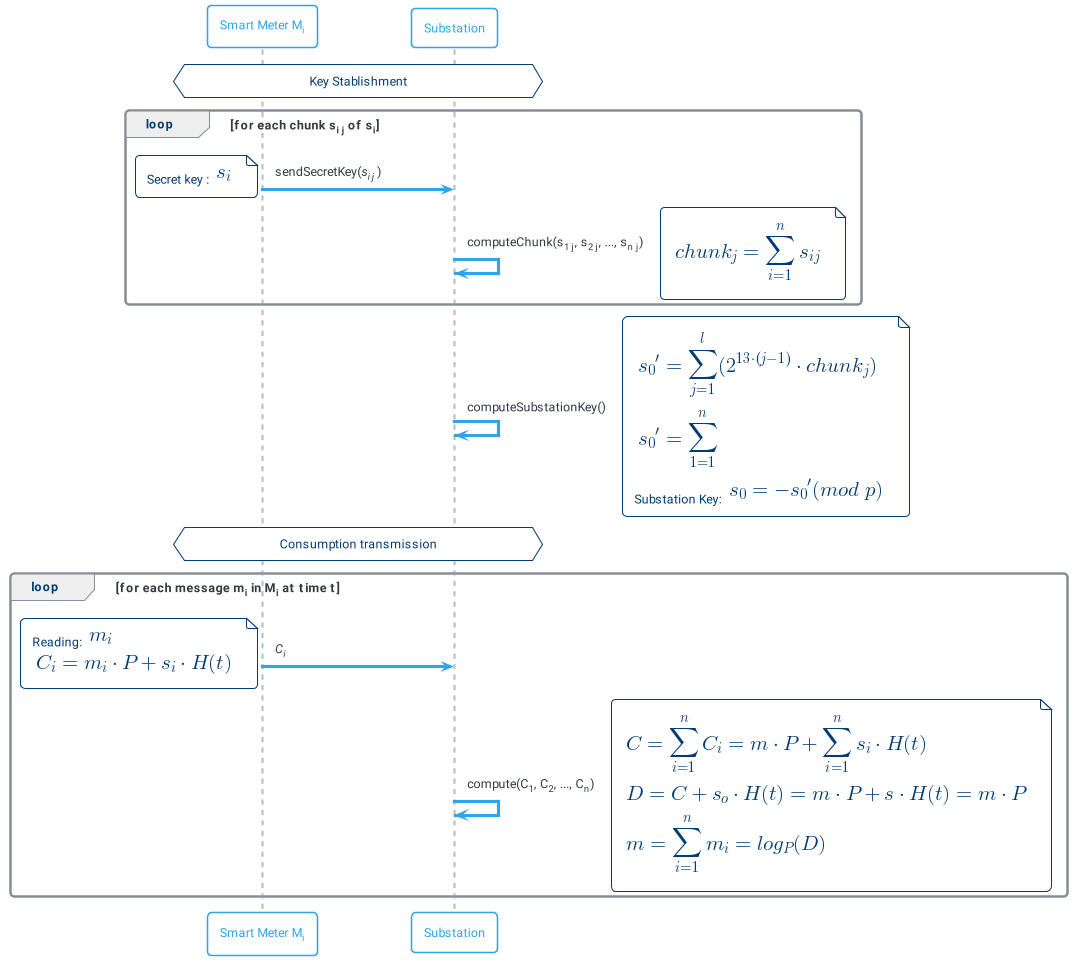
\includegraphics[width=16cm]{umls/recsi.png}
	\caption{Diagrama de seqüència del protocol RECSI}
\end{figure}
\subsubsection{Configuració}
Abans d'engegar el sistema, es necessita que tant els comptadors com la subestació utilitzin el mateix cos i element generador per tal de xifrar i desxifrar correctament els missatges. Per tant, s'haurà d'elegir:
\begin{itemize}
	\item Corba el·líptica $E$ definida sobre un cos primer $F_q$ d'ordre $p$ d'almenys 256 bits.
	\item Un punt $P \in E(F_q)$, que serà l'element generador de la corba.
\end{itemize}
A més a més, es necessitarà l'ús d'una funció \textit{hash}\footnote{
Una funció \textit{hash} és tota aquella funció que pot ser utilitzada per transformar un conjunt d'elements en un altre, on aquest últim té una cardinalitat establerta.
}
$H$ que retorni un punt $Q \in E(F_q)$ donat un element $e \in F_q$. Això ens permetrà operar amb elements discrets com si fossin punts de la corba. 
\subsubsection{Establiment de claus}\label{section:ks}
La configuració de les claus s'ha de realitzar a l'inici del sistema i cada cop que hi hagi un canvi en el conjunt de comptadors del barri, per exemple, quan s'afegeix o s'elimina un comptador.
\\
\\
Les claus dels comptadors $s_i$ formaran part de la clau privada de la subestació $s_0$. La seva relació serà semblant al exemple explicat en la \textit{Secció \ref{subsec:homomorfism-exemple}}. Aquesta clau es farà servir per trobar el consum total del barri un cop agrupats els valors xifrats.
La clau generada per cada comptador ha de ser d'una llargada similar a l'ordre del cos $F_q$, és a dir, $p$.
\begin{enumerate}
	\item Cada comptador $M_i$ generarà el seu secret $s_i < p$. Aquesta serà dividida en $l$ \textit{chunks} de, com a màxim, 13 bits, de manera que:
	\[s_i = (s_{il}\ ||\ \dots ||\ s_{i_2}\ ||\ s_{i1})\]
	Es requereix que $13 \cdot l$ sigui igual o més gran que la llargada en bits de $p$. Per tal de passar-ho de manera segura sense que la subestació pugui saber una part del secret del comptador, es realitza  $l$ vegades el protocol de Busom \cite{busom}.
	\item Després de cada execució $j \ , \ \ 1 \le j \le l$ del pas 1, la subestació realitza el sumatori de la mateixa part $j$ en totes les claus, de manera que troba:
	\[s_{1j} + s_{2j} + \dots + s_{nj} = \sum_{i=1}^{n} s_{ij}\]
	\item Un cop calculats tots els \textit{chunks} resultants, la subestació computa:
	\[s_0^{'} = \sum_{j=1}^{l} \Big( 2^{13 \cdot (j - 1)} \cdot \sum_{i=1}^{n} s_{ij} \Big) = \sum_{i=1}^{n} s_i\]
	D'aquesta manera, usant el protocol de Busom, la subestació no pot saber un chunk del secret d'un comptador sinó el valor resultant dels secrets. Un cop sabent $s_o^{'}$, la subestació defineix la seva clau secreta com:
	\[s_0\ =\ - s_0^{'} \ (mod \ p)\]
\end{enumerate}
\subsubsection{Transmissió del consum}\label{section:ct}
La transmissió dels comptadors intel·ligents a la subestació es realitza de manera regular a cada interval de temps. A cada ronda $t \in \mathbb{Z^+}$, cada comptador intel·ligent $M_i$ enviarà el seu consum $m_i$ a la subestació $SSt$. Un cop realitzada la transmissió, el valor $t$ incrementarà en un. El procediment a seguir és el següent:
\begin{enumerate}
	\item Cada comptador $M_i$ transmet la seva lectura $m_i$ trobant un punt de la corba el·líptica $C_i$ tal que:
	\[C_i = m_i \cdot P + s_i \cdot H(t)\]
	\item Un cop la subestació rep tots els punts de cada comptador intel·ligent, els agrega per tal de obtenir un punt resultant $C$:
	\[C = \sum_{i=1}^{n}m_i = m \cdot P + \sum_{i=1}^{n}s_i \cdot H(t) = m \cdot P + s_0^{'}\cdot H(t)\]
	\item La subestació, per tal d'obtenir un punt $D$ que només depengui sobre $P$ i el missatge, utilitza la seva clau secreta per eliminar el soroll produït per les claus secretes dels comptadors:
	\[D = C + s_0 \cdot H(t) = m \cdot P + \big( s_0^{'} + s_0 \big) \cdot H(t) = m \cdot P\]
	\item Finalment, la subestació haurà de computar el logaritme discret de $D$ en base $P$ per tal d'obtenir la lectura resultant del barri.
	\[m = \sum_{i=1}^{n} m_i = log_P(D)\]
	Com més curts siguin els intervals de temps, més petit serà el valor del consum de cada comptador. Això implica una computació no tan costosa de l'algorisme de Pollards Lambda, o d'altres que sol·lucionin el logaritme discret.
\end{enumerate}

\newpage\part{Disseny de la implementació}\label{part:disseny}
\subfile{sec/disseny.tex}
\part{Anàlisis}\label{part:analisis}
\subsection{Algorismes de computació del logaritme discret}

\bibliography{document}
\bibliographystyle{unsrt}

\end{document}
